\chapter{Materials and Methods} \label{chap:Materials_and_Methods}

\section{Data and Pipeline}

The tools listed in \autoref{tab:Package_Version} were installed using the \texttt{Conda package distribution system} version 2-2.4.0 \autocite{anaconda_software_distribution_anaconda_2020}. A configuration file for recreation of the used environment is present in the projects GitHub repository\footnote{\url{https://github.com/ahenoch/Masterthesis.git}}

\begin{table}[hbt]
    \footnotesize
    \centering
    \caption[Pipeline tools]{\textbf{Pipeline tools.} All packages used in the project are listed here.}
    \label{tab:Package_Version}
    \begin{tabular*}{0.75\textwidth}{@{\extracolsep{\fill}\hspace{6pt}}llll}
        \toprule
        \textbf{Name} & \textbf{Version} & \textbf{Purpose} & \textbf{Source}\\
        \midrule
        \texttt{BioPython} & 1.78 & alignments and tree construction & \autocite{cock_biopython_2009}\\
        \texttt{ETE3} & 3.1.2 & tree plotting and labeling & \autocite{huerta-cepas_ete_2016}\\
        \texttt{HDBSCAN} & 0.8.26 & hybrid vector clustering & \autocite{mcinnes_hdbscan_2017}\\
        \texttt{kneed} & 0.7.0 & Kneedle Algorithm implementation & \autocite{satopaa_finding_2011}\\
        \texttt{MAFFT} & 7.475 & \acrlong{MSA} & \autocite{katoh_mafft_2013}\\
        \texttt{numpy} & 1.19.5 & matrix and vector calculations & \autocite{harris_array_2020}\\
        \texttt{pandas} & 1.2.2 & dataframe creation and management & \autocite{mckinney_data_2010}\\
        \texttt{seaborn} & 0.11.1 & plotting and data visualization & \autocite{waskom_seaborn_2021}\\
        \texttt{scikit-learn} & 0.24.1 & \texttt{PCA} and vector normalization & \autocite{pedregosa_scikit-learn_2011}\\
        \texttt{SciPy} & 1.6.0 & vector distance calculations & \autocite{scipy_10_contributors_scipy_2020}\\
        \texttt{UMAP} & 0.4.6 & \texttt{UMAP} dimension reduction & \autocite{mcinnes_umap_2020}\\
        \bottomrule
    \end{tabular*}
\end{table}

Since its file size exceeds the limits of GitHub, the FASTA file containing all the sequences of the \gls{IAV}, that are used in this project is only present on the attached USB stick, also containing a copy of the projects repository. The FASTA file can be manually retrieved from the \gls{IRD}\footnote{\url{https://www.fludb.org/brc/home.spg?decorator=influenza}} using the settings in \autoref{tab:Search} for nucleotide sequence search. The header of the FASTA file has to be formatted as Accession Number, Strain Name, Segment, Protein Symbol, Type, SubType, Date, Host Species, Curation Flag in the given order before downloading from \gls{IRD} for the tool to work as expected.

\vspace{1em}

The version used for the proposed results was acquired at 08/11/2020\footnote{GenBank Genome Sequence/Annotation Update <= 11/2020}. Newer versions\footnote{GenBank Genome Sequence/Annotation Update >= 05/2021} might change the results slightly.

\begin{table}[!hbt]
    \footnotesize
    \centering
    \caption[Search parameter]{\textbf{Search parameter.} The parameters to use on the nucleotide sequence search interface of the \gls{IRD}.}
    \label{tab:Search}
    \begin{tabular*}{0.5\textwidth}{@{\extracolsep{\fill}\hspace{6pt}}ll}
        \toprule
        \textbf{Field} & \textbf{Parameter}\\
        \midrule
        Data Type & Genome Segments\\
        Virus Type & A\\
        Complete Genome & Complete Genome Only\\
        Select Segments & All\\
        Complete & All\\
        \bottomrule
    \end{tabular*}
\end{table}

\begin{table}[!hbt]
    \footnotesize
    \centering
    \caption[Summary of the clustering methods]{\textbf{Summary of the clustering methods.} For easier separation the different settings were listed. Method PCA/DBCV and PCA/Knee use \autoref{fig:Vectorization_Pipeline} pathway \textsf{\textbf{1}} followed by \autoref{fig:Clustering_Pipeline} pathway \textsf{\textbf{3}} for method PCA/DBCV and \textsf{\textbf{4}} for PCA/Knee. Method UMAP/DBCV and UMAP/Knee differ only by the first part using \autoref{fig:Vectorization_Pipeline} pathway \textsf{\textbf{2}} instead of \textsf{\textbf{1}}.}
    \label{tab:methods}
    \begin{tabular*}{\textwidth}{@{\extracolsep{\fill}\hspace{6pt}}lllll}
        \toprule
        \textbf{Abbreviation} & \textbf{Method} & \textbf{100 Components} & \textbf{30 Components} & \textbf{Exploration}\\
        \midrule
        PB & PCA/DBCV & --- & PCA & DBCV\\
        PK & PCA/Knee & --- & PCA & Kneedle Algorithm\\
        UD & UMAP/DBCV & PCA & UMAP & DBCV\\
        UK & UMAP/Knee & PCA & UMAP & Kneedle Algorithm\\
        \bottomrule
    \end{tabular*}
\end{table}

In this project four different ways to cluster the segments of \gls{IAV} are described and discussed (\autoref{tab:methods}). The methods are compared to each other and analyzed for their capability of \gls{IAV} clustering. Abbreviations of the four methods were used in the following as indicated in \autoref{tab:methods}.%Two 

\vspace{1em}

A combined version of the pipelines in \autoref{fig:Vectorization_Pipeline}, \autoref{fig:Clustering_Pipeline} and \autoref{fig:Tree_Pipeline} is available in the projects GitHub repository\footnote{\url{https://github.com/ahenoch/Masterthesis.git}} as a novel clustering tool for \gls{IAV} genomes. The tool contains the method elaborated as best suitable for \gls{IAV} clustering and is intended to be used for future research (\autoref{sec:Serotype_Classification}).

\begin{figure}[!hbt]
    \centering
    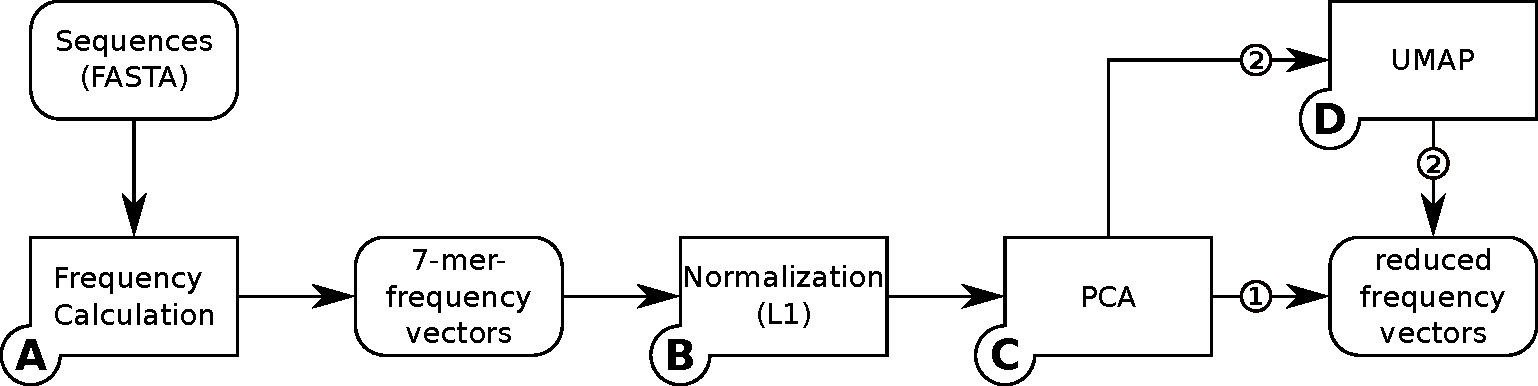
\includegraphics[width=\textwidth]{Graphics/Vectorization.pdf}
    \caption[Preprocessing pipeline]{\textbf{Preprocessing pipeline.} To create high-quality vectors representing the sequences, the FASTA file was translated to normalized vectors containing the 7-mer frequencies of the specific sequences (\textsf{\textbf{A}} and \textsf{\textbf{B}}). By pathway \textsf{\textbf{1}}, a low complexity representation of the vectors is obtained for clustering only using \texttt{PCA} (\textsf{\textbf{C}}). Pathway \textsf{\textbf{2}} describes additional execution of \texttt{UMAP} that can be used after \texttt{PCA} as intermediate instead of final step (\textsf{\textbf{D}}). Reduction with pathway \textsf{\textbf{1}} or \textsf{\textbf{2}} results in reduced frequency vectors with 30 components.} 
    \label{fig:Vectorization_Pipeline}
\end{figure}

\begin{figure}[!hbt]
    \centering
    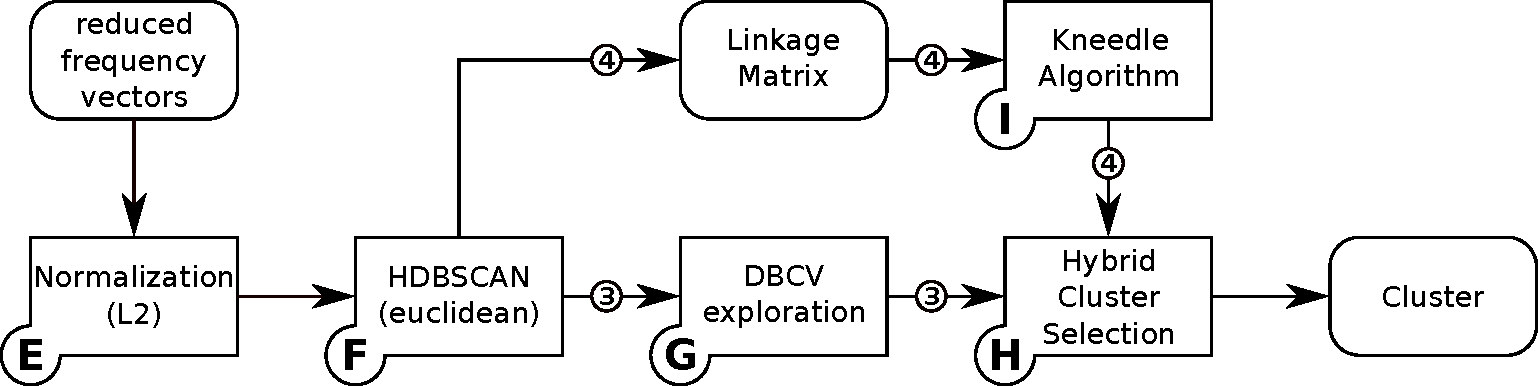
\includegraphics[width=\textwidth]{Graphics/Clustering.pdf}
    \caption[Clustering pipeline]{\textbf{Clustering pipeline.} Following the preprocessing pipeline (\autoref{fig:Vectorization_Pipeline}) normalization is used again with L2-norm as preparation for \texttt{HDBSCAN} (\textsf{\textbf{E}}). Initial \texttt{HDBSCAN} clustering (\textsf{\textbf{F}}) is performed in preparation to the $\varepsilon$ exploration using either pathway \textsf{\textbf{3}} or \textsf{\textbf{4}}. Final hybrid clustering (\textsf{\textbf{H}}) is then executed on the results of the $\varepsilon$ exploration using the Kneedle Algorithm (\textsf{\textbf{I}} and pathway \textsf{\textbf{4}} or DBCV (pathway \textsf{\textbf{3}} and \textsf{\textbf{G}}).}
    \label{fig:Clustering_Pipeline}
\end{figure}

\begin{figure}[!hbt]
    \centering
    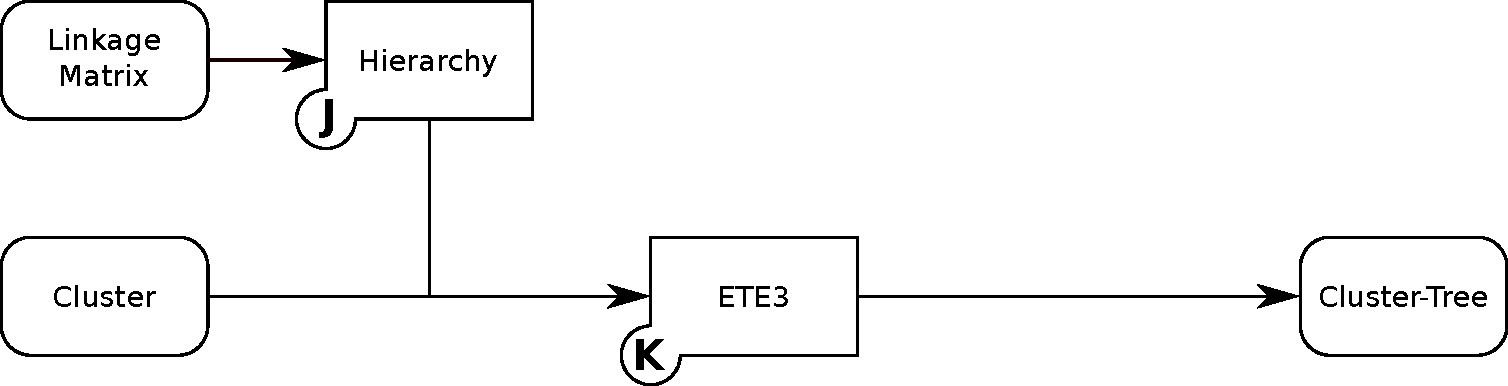
\includegraphics[width=\textwidth]{Graphics/Tree.pdf}
    \caption[Postprocessing pipeline]{\textbf{Postprocessing pipeline.} Following the clustering pipeline (\autoref{fig:Clustering_Pipeline}) the cluster-tree is build by \texttt{BioPython} and visualized by \texttt{ETE3} (\textsf{\textbf{J}}). For every cluster the vectors with the smallest distance to the other cluster members are calculated and determined as the clusters centroids (\textsf{\textbf{K}}).}
    \label{fig:Tree_Pipeline}
\end{figure}

Execution of the tool on the FASTA file containing 449462 sequences takes around one and a half hours. The sequences are, thereby, clustered segment-wise based on their 7-mer frequencies. The output consists of database ready CSV files holding the cluster assignment of every sequence, analysis graphics and a labeled cluster tree of each used segment. 

\vspace{1em}

The method is based on the one proposed by \textcite{viehweger_addressing_2019}. Instead of using the tool \texttt{nanotext} as proposed in \textcite{viehweger_encoding_2019}, a simple 7-mer frequency calculation was implemented and used as described in \autoref{sec:Frequency}. Similar to \textcite{viehweger_addressing_2019}, the calculated vectors were clustered using \texttt{HDBSCAN} with custom settings described in the \autoref{sec:HDBSCAN}. Since \texttt{nanotext} was not used in this project, different types of dimension reduction were performed and compared, as described in \autoref{sec:PCA} and discussed in \autoref{sec:Clustering}. With reference to the use of cosine similarity $s_{\text{cos}}(\mathbf{x}, \mathbf{y})$ as measurement for genomic similarity in \texttt{nanotext}, the use of the complementary cosine distance $d_{\text{cos}}(\mathbf{x}, \mathbf{y})$ in \texttt{HDBSCAN} was targeted (\autoref{eq:cos}) \autocite{viehweger_encoding_2019}. %To my best knowledge there is no other publication to the present day that used the same method proposed or created similar results.

\begin{equation}\label{eq:cos}
    \begin{aligned}
        d_{\text{cos}}(\mathbf{x}, \mathbf{y}) = 1 - s_{\text{cos}}(\mathbf{x}, \mathbf{y})
    \end{aligned}
\end{equation}

\section{7-mer Frequency Calculation} \label{sec:Frequency}

The FASTA file containing the genomes of \gls{IAV} for clustering, was converted to vectors to enable clustering in high dimension by counting their 7-mer frequency (\autoref{fig:Vectorization_Pipeline} \textsf{\textbf{A}}). $4^7$ possible constellations of the nucleotides A,C,G,T with length 7 exist. Therefore, taking every constellation into consideration, the vector of every sequence has $4^7$ components. The numbers in the vector components are the number of occurrences of the related 7-mer in the sequence. The first constellation of the $4^7$ possible ones with length 7 is AAAAAAA, given a example sequence of the FASTA contains this 7-mer 10 times, the first component of the sequences vector would be 10. \autoref{fig:k-mer} illustrates the calculation using 3-mers instead of 7-mers.

\begin{figure}[!hbt]
    \centering
    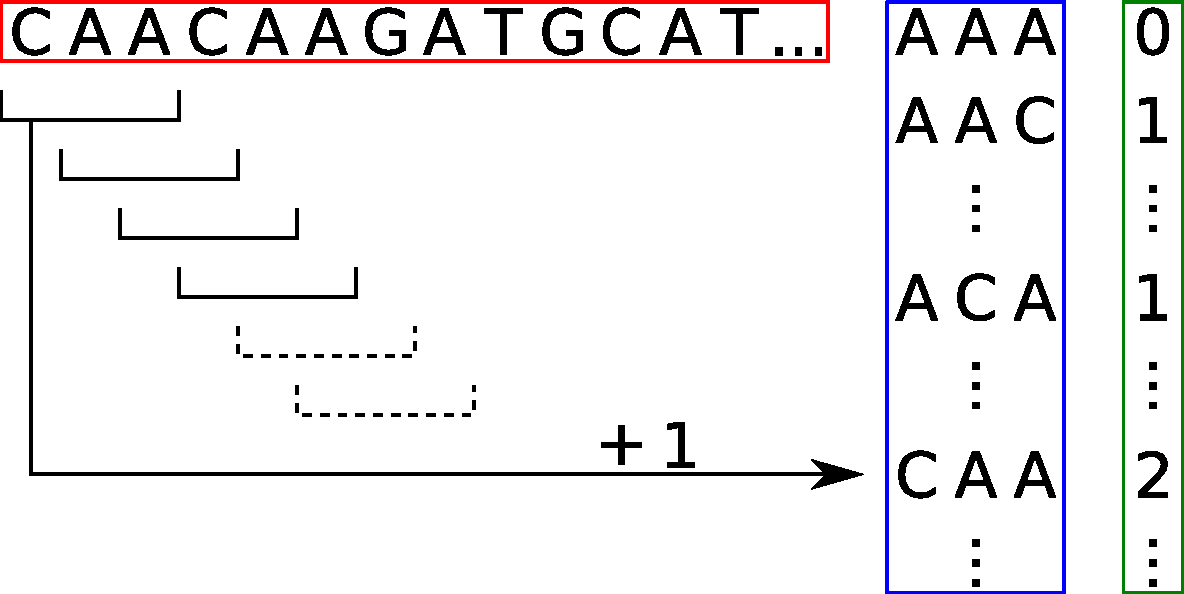
\includegraphics[width=0.5\textwidth]{Graphics/Kmer.pdf}
    \caption[K-mer vector creation]{\textbf{K-mer vector creation.} An example genomic sequence (red box) is splitted into 3-mers. The sequences 3-mers are then compared to the list of all $4^3$ possible 3-mer constellations (blue box) Based on the occurrence number of the lists 3-mers in the sequence a vector with $4^3$ components is created (green box).}
    \label{fig:k-mer}
\end{figure}

To gain the frequency of the 7-mers all the vectors were normalized to a vector sum of 1, according to L1-norm (\autoref{eq:norm1} and \autoref{fig:Vectorization_Pipeline} \textsf{\textbf{B}}). 

\begin{equation}\label{eq:norm1}
    \begin{aligned}
        \mathbf{\hat{x}} = \frac{\mathbf{x}}{\Vert\mathbf{x}\Vert_1}
    \end{aligned}
\end{equation}

\section{Dimension Reduction} \label{sec:PCA}

\texttt{PCA} was used to handle the complexity of the vectors by simplification with the least loss of information possible (\autoref{fig:Vectorization_Pipeline} \textsf{\textbf{C}}) \autocite{pearson_liii_1901} \autocite{pedregosa_scikit-learn_2011}.

\vspace{1em}

Without posterior use of \texttt{UMAP} 30 components were extracted by the \texttt{PCA} (\autoref{fig:Vectorization_Pipeline} pathway \textsf{\textbf{1}}) and otherwise 100 (\autoref{fig:Vectorization_Pipeline} pathway \textsf{\textbf{2}}). Extraction of 30 or 100 components out of $4^7$ in total equals $\approx 0.18\%$ or $\approx 0.61\%$. The size limit of the \texttt{PCA} function for calculation with default setting \texttt{svd\_solver='auto'} is 500 different vectors with 500 components and at least 80\% of the components to extract. Since every maximum for standard settings was exceeded, \texttt{svd\_solver='randomized'} setting was used automatically. %\autocite{pedregosa_scikit-learn_2011}. %Randomized truncated \gls{SVD} is performed in the PCA as described in \textcite{halko_finding_2010}.

\vspace{1em}

\texttt{UMAP} was used for dimension reduction similar to \texttt{PCA}, aiming to better preserve the global structure of the data (\autoref{fig:Vectorization_Pipeline} \textsf{\textbf{D}} and pathway \textsf{\textbf{2}}) \autocite{mcinnes_umap_2020}. It is similar to the well-known \texttt{t-SNE} with better run time performance and better structure preservation in the lower dimension and less restrictions \autocite{maaten_visualizing_2008, mcinnes_umap_2020}. %Embedding is, hereby, the presentation of the used dataset in the lower dimension.

The used parameters of \texttt{UMAP} match most of the ones listed in the manual under section \glqq UMAP enhanced clustering\grqq{}\footnote{\url{https://umap-learn.readthedocs.io/en/latest/clustering.html} (accessed 07/01/2020)}. The settings are proposed to be used with \texttt{UMAP} prior to \texttt{HDBSCAN} clustering. Since the goal was clustering, not plotting 30 components was used instead of the proposed 2. The neighbors number was also changed. It is recommended to be set in a range of 1 to 100. Based on the high number of sequences used e.~g.~, 56617 for segment 4, the highest recommended setting of 100 was used to better preserve the global picture of the data. Also based on the input size \texttt{n\_epochs=200} setting was used automatically.

\vspace{1em}

\texttt{UMAP} was used posterior to dimension reduction with \texttt{PCA}, because of the similarity to \texttt{t-SNE}. As explained in the manual of \texttt{t-SNE}\footnote{\url{https://scikit-learn.org/stable/modules/generated/sklearn.manifold.TSNE.html} (accessed 07/01/2020)}, the dimension should be reduced to a reasonable amount prior to execution to reduce noise. In in section \glqq What is the difference between PCA / UMAP / VAEs?\grqq{} of the \texttt{UMAP} manual\footnote{\url{https://umap-learn.readthedocs.io/en/latest/faq.html} (accessed 07/01/2020)} a pipeline is proposed, to reduce from high dimension with \texttt{PCA}, continue with reduction by \texttt{UMAP} and cluster with \texttt{HDBSCAN} and is, therefore, used as reference. Reduction with \texttt{UMAP} to 30 components posterior to \texttt{PCA} with 100 components also provided a comfortable balancing of computational effort of both methods, while preserving $\approx 85\%$ explained variance with \texttt{PCA} \autocite{mcinnes_umap_2020}. 

\section{Hybrid Clustering} \label{sec:HDBSCAN}

\texttt{HDBSCAN} was used to cluster the reduced vectors. It is an clustering algorithm proposed by \textcite{campello_hierarchical_2015} as a novel version of the well-known \texttt{DBSCAN} \autocite{hutchison_density-based_2013}. Execution of \texttt{HDBSCAN} involves varying values of $\varepsilon$, thus, not one specific threshold is used to define the clusters, but instead clusters of varying densities are extracted based on their stability \autocite{mcinnes_hdbscan_2017}. \texttt{HDBSCAN} was used with hybrid clustering setting as proposed in \textcite{malzer_hybrid_2020}, combining \texttt{HDBSCAN} it with \texttt{DBSCAN}. Thereby, some of the disadvantages of using either of these methods can be avoided \autocite{mcinnes_hdbscan_2017, moulavi_density-based_2014}. Since \texttt{DBSCAN} is a hierarchical clustering tool, it is dependent on a strict threshold $\varepsilon$ for clustering. Vectors not surrounded by $k$ other vectors in a radius defined by this threshold value $\varepsilon$ are omitted as single vector clusters or noise \autocite{ester_density-based_1996, schubert_dbscan_2017}. Standard \texttt{HDBSCAN}, on the other hand, tend to create unwanted micro-clusters in areas of high density \autocite{mcinnes_hdbscan_2017}. Using the hybrid \texttt{HDBSCAN} proposed in \autocite{malzer_hybrid_2020}, a threshold value $\varepsilon$ can be used to extract these high density areas as single clusters with \texttt{DBSCAN}, but still use the standard \texttt{HDBSCAN} for the otherwise omitted vectors (\autoref{fig:Hybrid} and \autoref{fig:Clustering_Pipeline} \textsf{\textbf{H}}). Hybrid \texttt{HDBSCAN} is, thus, clustering with \texttt{DBSCAN},resulting in a \textbf{raw} cluster number containing finished clusters and omitted single vector clusters, and subsequent standard \texttt{HDBSCAN}, reducing the \textbf{final} cluster number by clustering the omitted vectors.

\begin{figure}[!hbt]
    \centering
    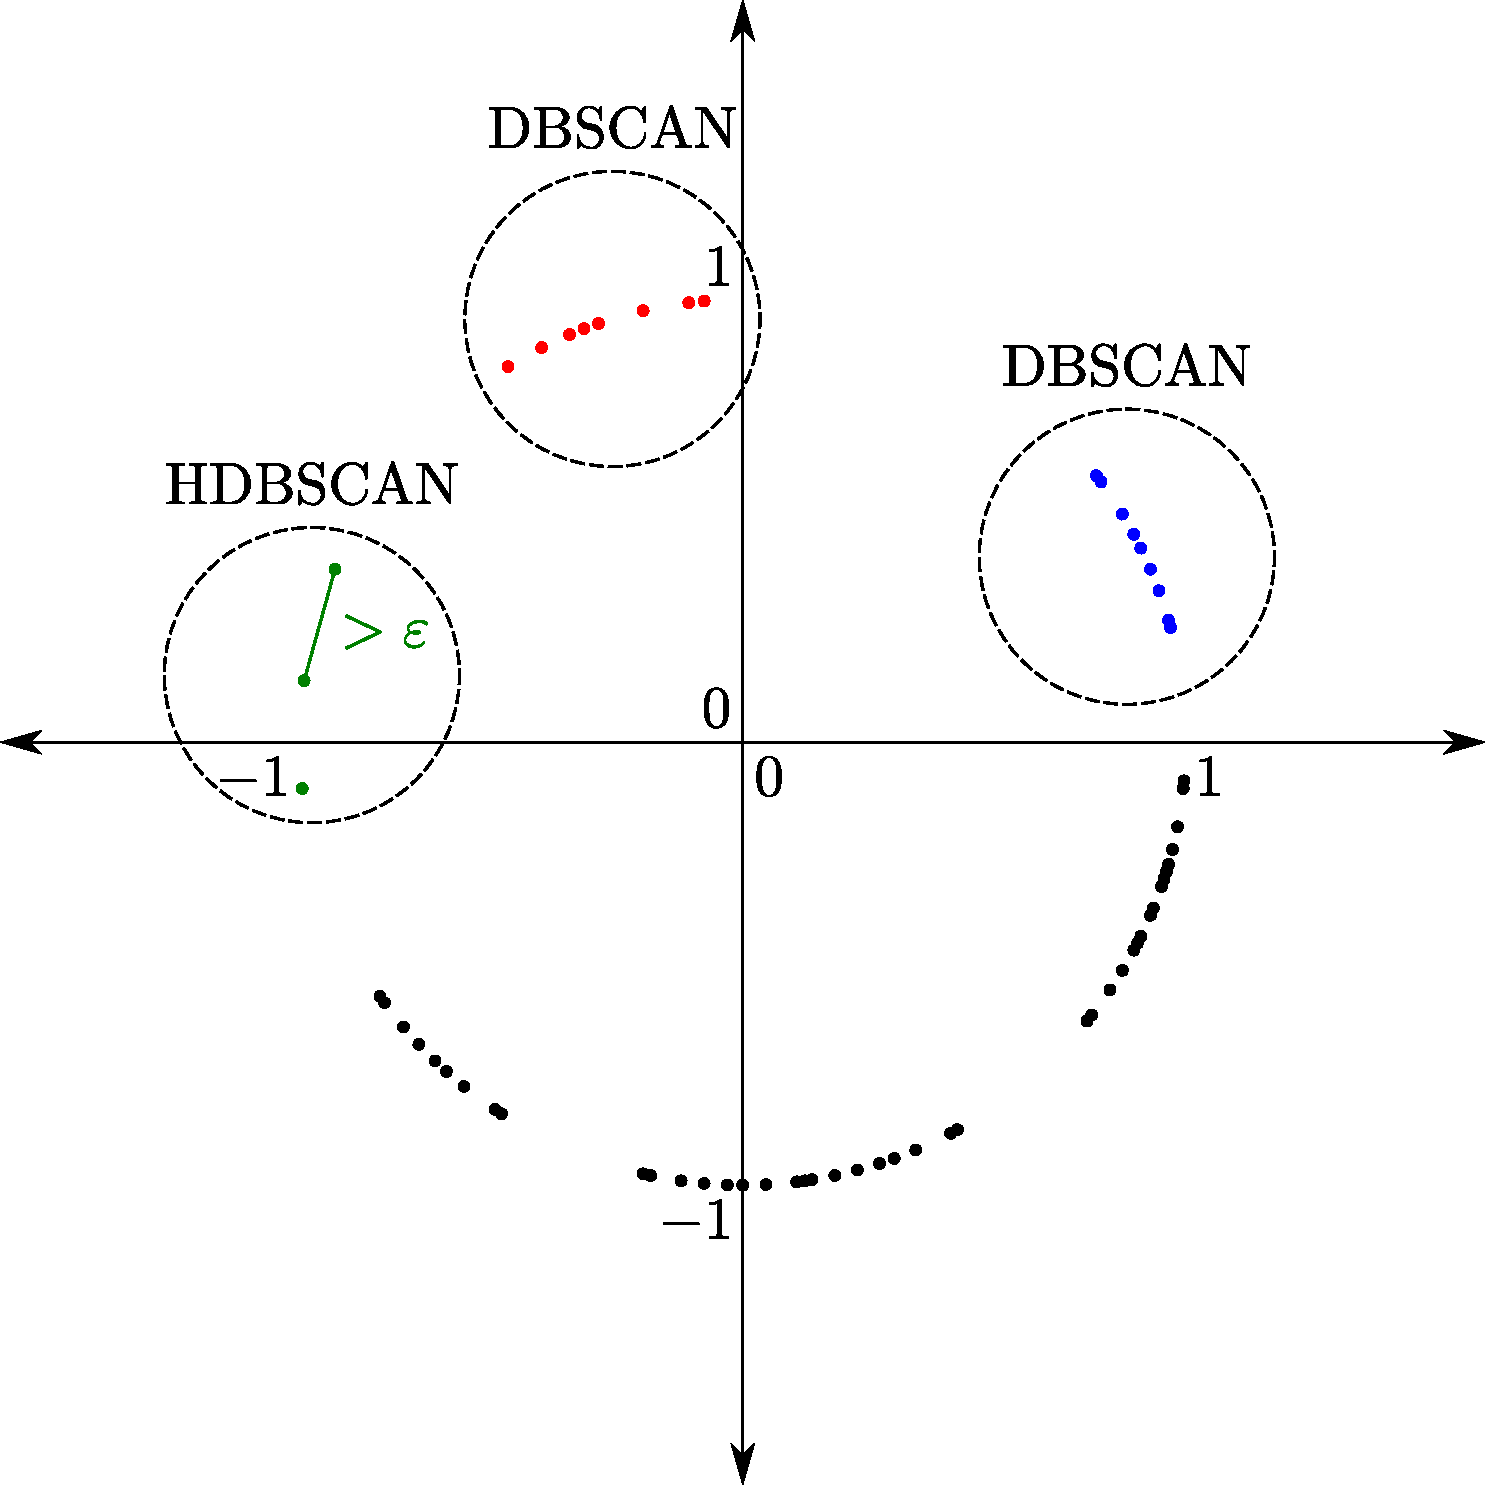
\includegraphics[width=\textwidth]{Graphics/Hybrid.pdf}
    \caption[Hybrid clustering threshold]{\textbf{Hybrid clustering threshold.} The hybrid clustering \texttt{HDBSCAN} differentiate between clusters where vectors are connected by distances smaller and higher than $\varepsilon$. When the distance is smaller, the \texttt{DBSCAN} algorithm is used and clusters are generated based on this threshold value $\varepsilon$ by combining vectors with smaller distance. Omitted vectors, not having a given number of $k=1$ vectors in reachable distance of $\varepsilon$ and are, therefore, impossible to be clustered by \texttt{DBSCAN} are subsequently clustered with \texttt{HDBSCAN} building clusters with higher threshold if appropriate. The graphic is based on \glqq Combining HDBSCAN* with DBSCAN\grqq{} in the manual\footnotemark and adapted to the calculations in this project, as a two dimensional example.}
    \label{fig:Hybrid}
\end{figure}

\footnotetext{\url{https://hdbscan.readthedocs.io/en/latest/how_to_use_epsilon.html}}
This method is useful when having a small cluster size value, while still aiming to cluster high-density areas together exactly suitable for the proposed clustering. Specific strains of \gls{IAV} are sequenced a lot more, thereby probably creating high-density areas that should be clustered together with \texttt{DBSCAN}. The small cluster size is, thereby, used to find small clusters of rare sequenced variants by \texttt{HDBSCAN}, with possibly important mutations in low-density areas \autocite{malzer_hybrid_2020}. As explained, the smallest minimum cluster size of 2 was used to capture, in the best case, even genomes with rare appearing mutations, in their own clusters. To declare as least vectors as possible as noise, the minimum samples value $k$ was also set to the minimum 1. Standard \texttt{HDBSCAN} was once performed without the hybrid setting, in preparation of $\varepsilon$ exploration as described in \autoref{sec:epsilon} \autoref{fig:Clustering_Pipeline} \textsf{\textbf{F}}). Hybrid \texttt{HDBSCAN} clustering was used with the same settings plus respective $\varepsilon$ value \autoref{fig:Clustering_Pipeline} \textsf{\textbf{H}}).

\vspace{1em}

Distance calculations by \texttt{HDBSCAN} were performed with the euclidean distance setting due to an open issue in the GitHub Repository of \texttt{HDBSCAN}\footnote{\url{https://github.com/scikit-learn-contrib/hdbscan/issues/69} (accessed 06/02/21)}. In the issue the inability to use cosine distance metric with \texttt{HDBSCAN} and the approximation of it by chord distance metric, is described. Given that chord distance metric is also not available firsthand, the possibility to use normalization of the vectors with L2-norm, prior to clustering with euclidean metric setting is also mentioned \autoref{fig:Clustering_Pipeline} \textsf{\textbf{E}}). 

\begin{figure}[!hbt]
    \centering
    \begin{subfigure}[b]{0.475\textwidth}
        \caption[Chord]{\textbf{Chord distance}}
        \label{subfig:Chord}
        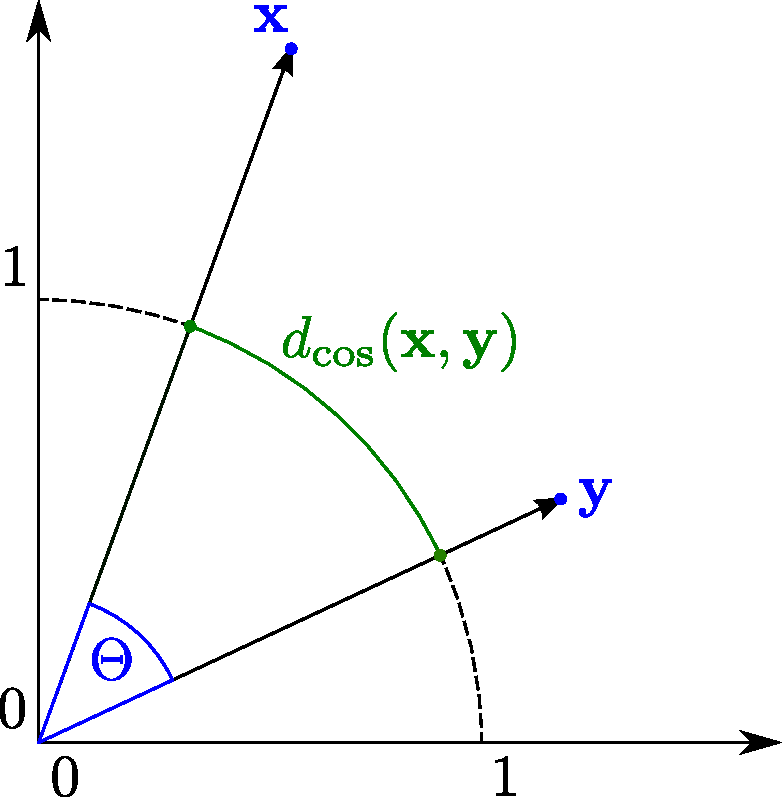
\includegraphics[width=\textwidth]{Graphics/Chord.pdf}
    \end{subfigure}
    \hfill
    \begin{subfigure}[b]{0.475\textwidth}
        \caption[L2]{\textbf{L2-norm normalized euclidean distance}}
        \label{subfig:L2}            
        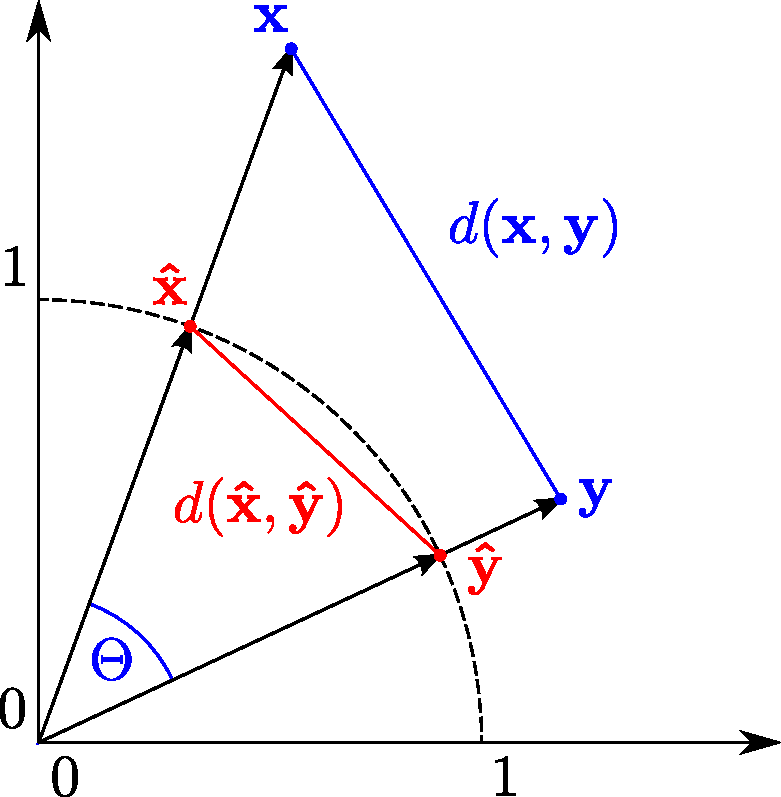
\includegraphics[width=\textwidth]{Graphics/L2.pdf}
    \end{subfigure}
    \caption[Chord calculation background]{\textbf{Chord calculation background.} The chord can be calculated with the radius similar for both vectors and the information of the angle of two vectors to the origin of the coordinate system. Since this information is not always available or sometimes expensive to calculate for a high number of vectors, the euclidean distance can be used with a L2-norm of both vectors equal to $r$ for similar results instead. To approximate cosine distance, the same calculation of euclidean distance is used with L2-norm equal to $r = 1$. To always obtain similar values of L2-norm equal to 1, L2-norm normalization is used on every vector.}
    \label{fig:L2_Normalisation_Background}
\end{figure}

\begin{equation}\label{eq:norm2}
    \begin{aligned}
        \mathbf{\hat{x}} = \frac{\mathbf{x}}{\Vert\mathbf{x}\Vert_2}
    \end{aligned}
\end{equation}

Calculation of chord distance $d_{\text{chord}}$ is possible when having two vectors, here as an example named as $\mathbf{a}$ and $\mathbf{b}$ with the same L2-norm equal to a radius $r$ of a sphere centered to the origin of the coordinate system and an angle of $\Theta$ (\autoref{eq:chord1} and \autoref{subfig:Chord}) \autocite{maor_trigonometric_2013}. The euclidean distance $d_{\text{eucl}}$ is equal to the chord distance for the same vectors.

\begin{equation}\label{eq:chord1}
    \Vert\mathbf{a}\Vert_2 = \Vert\mathbf{b}\Vert_2 = r \Rightarrow 
    \begin{aligned}
        d_{\text{chord}}(\mathbf{a},\mathbf{b}) &= 2 \cdot r \sin \left(\frac{\Theta}{2}\right)\\
        &= d_{\text{eucl}}(\mathbf{a},\mathbf{b})
    \end{aligned}
\end{equation}

Thus, in this project, chord distance can be calculated with the euclidean distance metric, posterior to the normalization with the L2-norm, which scales the vectors to the unit sphere \autoref{subfig:L2}. 

\begin{equation}\label{eq:chord2}
    \Vert\mathbf{\hat{x}}\Vert_2 = \Vert\mathbf{\hat{y}}\Vert_2 = 1 \Rightarrow 
    \begin{aligned}
        d_{\text{chord}}(\mathbf{\hat{x}},\mathbf{\hat{y}}) &= d_{\text{eucl}}(\mathbf{\hat{x}},\mathbf{\hat{y}})\\
        &= \Vert\mathbf{\hat{x}} - \mathbf{\hat{y}}\Vert_2
    \end{aligned}
\end{equation}

The calculation of the chord distance, by L2-norm normalized vectors euclidean distance, is, thereby, integrated into the mutual reachability distance calculation of \texttt{HDBSCAN}. The mutual reachability distance is the maximum of the chord distance and the core distances of two vectors (\autoref{eq:reach}). The core distance is the minimum radius necessary to include 5 other vectors around a given vector \autocite{mcinnes_hdbscan_2017}. Threshold $\varepsilon$ is used on the mutual reachability distances between the vectors \autoref{fig:Hybrid}. 

\begin{equation}\label{eq:reach}
    \begin{aligned}
        d_{\text{mreach}-k}(\mathbf{\hat{x}},\mathbf{\hat{y}}) &= \max \{ \text{core}_k(\mathbf{\hat{x}}), \text{core}_k(\mathbf{\hat{y}}), d_{\text{eucl}}(\mathbf{\hat{x}},\mathbf{\hat{y}}) \}
    \end{aligned}
\end{equation}

The used chord distance is proportional with the initially intended to use cosine distance as shown in \autoref{eq:chord3}. Dividing the squared chord distance by 2 results in the cosine distance of the vectors \autoref{fig:Normalisation_Methods}.

\begin{equation}\label{eq:chord3}
    \Vert\mathbf{\hat{x}}\Vert_2 = \Vert\mathbf{\hat{y}}\Vert_2 = 1 \Rightarrow 
    \begin{aligned}  
        d_{\text{chord}}(\mathbf{\hat{x}},\mathbf{\hat{y}})^2 &= \Vert\mathbf{\hat{x}} - \mathbf{\hat{y}}\Vert_2^2\\
        &= (\mathbf{\hat{x}} - \mathbf{\hat{y}})^\top (\mathbf{\hat{x}} - \mathbf{\hat{y}})\\
        &= \mathbf{\hat{x}}^\top \mathbf{\hat{x}} - 2 \mathbf{\hat{x}}^\top \mathbf{\hat{y}} + \mathbf{\hat{y}}^\top \mathbf{\hat{y}}\\
        &= 2 - 2\mathbf{\hat{x}}^\top \mathbf{\hat{y}}\\
        &= 2 - 2 \cos(\Theta)\\
        &= 2 \cdot (1 - \cos(\Theta))\\
        &= 2 \cdot d_{\text{cos}}(\mathbf{\hat{x}},\mathbf{\hat{y}})
    \end{aligned}
\end{equation}

\begin{figure}[!hbt]
    \centering
    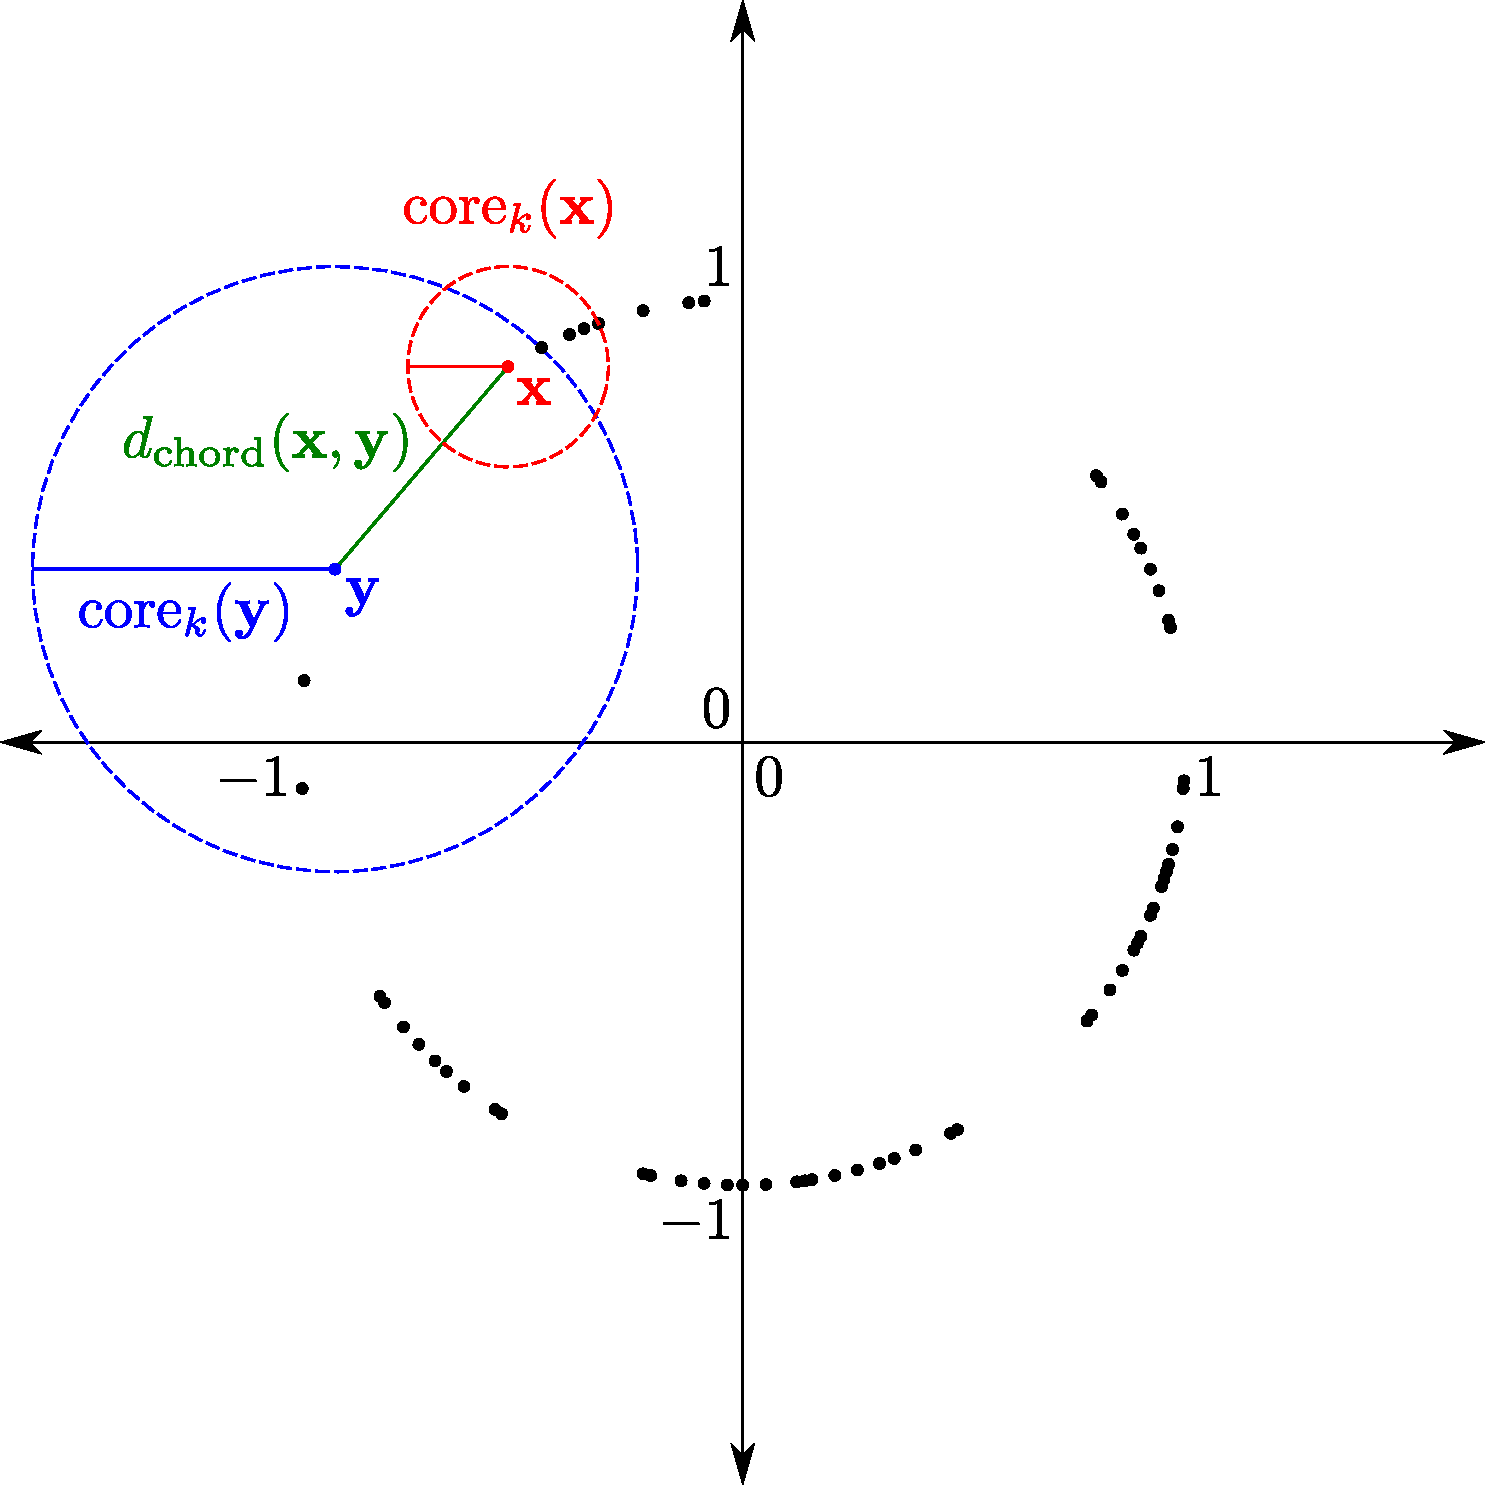
\includegraphics[width=\textwidth]{Graphics/HDB.pdf}
    \caption[Mutual reachability calculation]{\textbf{Mutual reachability calculation.} A low dimension representation of the calculation \texttt{HDBSCAN} performed in this project. To calculate the mutual reachability distance, the smallest radius is calculated to include exactly $k$ vectors. This example should demostrate the calculation for vector $\mathbf{x}$ in blue and $\mathbf{y}$ in red, with a $k$ of 5. The euclidean distance between these vectors is then calculated and compared to the radii. The maximum of both radii and the euclidean distance is the mutual reachability distance (\autoref{eq:reach}).}
    \label{fig:HDB}
\end{figure}

\section{Epsilon Selection} \label{sec:epsilon}

To find an appropriate value for $\varepsilon$, two different methods were used and compared (\autoref{fig:Clustering_Pipeline} pathway \textsf{\textbf{3}} and \textsf{\textbf{4}}). The first method, the \gls{DBCV} exploration in \autoref{fig:Clustering_Pipeline} \textsf{\textbf{G}}, is based on repeated execution of hybrid \texttt{HDBSCAN} with different settings for $\varepsilon$ and comparison by the \gls{DBCV}. The \gls{DBCV} is a calculation based on the minimum spanning tree to estimate overall cluster density \autocite{moulavi_density-based_2014}. To enable the calculation hybrid \texttt{HDBSCAN} was performed with \texttt{gen\_min\_span\_tree=True} setting.

\vspace{1em}

Second method for $\varepsilon$ exploration was performed using the Kneedle Algorithm on the linkage matrix created by the initially performed of standard \texttt{HDBSCAN} clustering (\autoref{fig:Clustering_Pipeline} \textsf{\textbf{F}} and \textsf{\textbf{I}}) \autocite{satopaa_finding_2011}. With increasing cluster number, the distance threshold $\varepsilon$ of hierarchical clustering decreases. This describes a decreasing curve of convex type with distance threshold on the y- and cluster number on the x-axis. The knee is the number of clusters at the point in the polynomial representation of the curve with maximal acceleration. Polynomial representation was used to find the maximum acceleration of the smoothed curve. Therefore the settings \texttt{curve='concave'}, \texttt{direction='increasing'} and \texttt{interp\_method='interp1d'} were used to find the optimal number of clusters. The optimal number of clusters was converted to the respective $\varepsilon$ threshold.

\vspace{1em}

Knee point selection was restricted to a given area between one and a maximum value of 500. The maximum was chosen to include the area with the highest expected differences. The best Knee point was expected to be less than 100, a higher value was used to prevent forcing the number of clusters to be maximal 100. 

\section{Alignments and Vector Calculations} \label{sec:MAFFT}

The labeled cluster trees were created by \texttt{ETE3} with a newick file, generated according to a feature request, proposed for the \texttt{SciPy}\footnote{\url{https://github.com/scipy/scipy/issues/8274} (accessed 06/02/21)} (\autoref{fig:Tree_Pipeline} \textsf{\textbf{J}}) \autocite{huerta-cepas_ete_2016}. Clusters centroid vectors were selected by calculating euclidean distance between all the vectors of a cluster to each other. The vector with the smallest mean distance was declared as centroid (\autoref{fig:Tree_Pipeline} \textsf{\textbf{K}}). 

%The materials described in the following were only used for the centroid guide tree creation and the analyses on H13/H16 sequences in the \autoref{sec:Clustering_Anomalies} to \autoref{sec:Dimension_Reduction} and are, therefore, not included in the novel \gls{IAV} clustering tool (\autoref{fig:Alignment_Pipeline} and \autoref{fig:Precalc_Pipeline}).

\begin{figure}[!hbt]
    \centering
    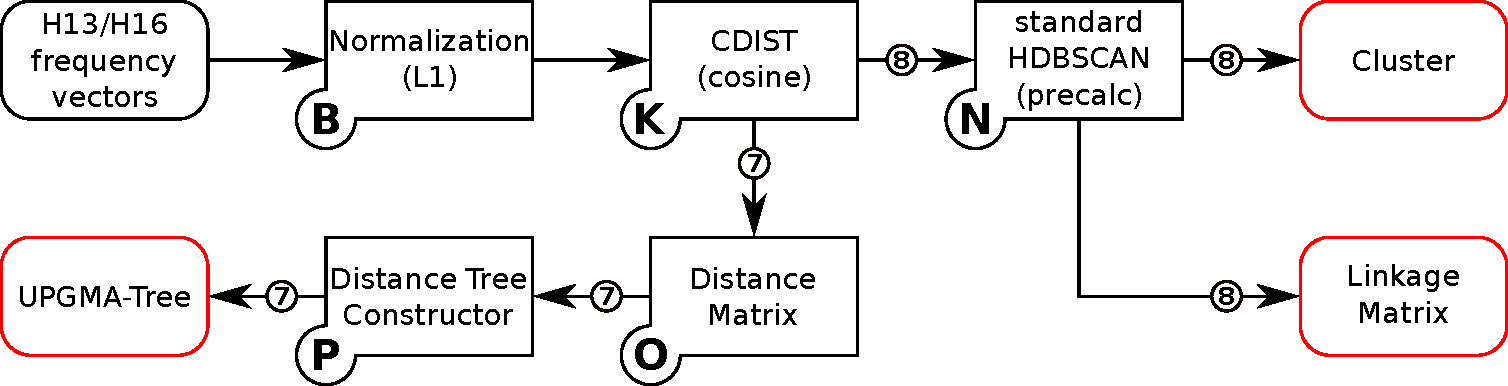
\includegraphics[width=\textwidth]{Graphics/Precalculated.pdf}
    \caption[Precalculation pipeline]{\textbf{Precalculation pipeline.} For the precalculated trees the L1-normalized 7-mer vectors distances were calculated and used for clustering by \texttt{HDBSCAN} (\textsf{\textbf{B}}, \textsf{\textbf{K}}, \textsf{\textbf{N}} and pathway \textsf{\textbf{7}}) and on the other hand processed with \texttt{BioPython} for \gls{UPGMA} tree creation and visualization by \texttt{ETE3} (\textsf{\textbf{N}} and \textsf{\textbf{8}}).}
    \label{fig:Precalc_Pipeline}
\end{figure}

\begin{figure}[!hbt]
    \centering
    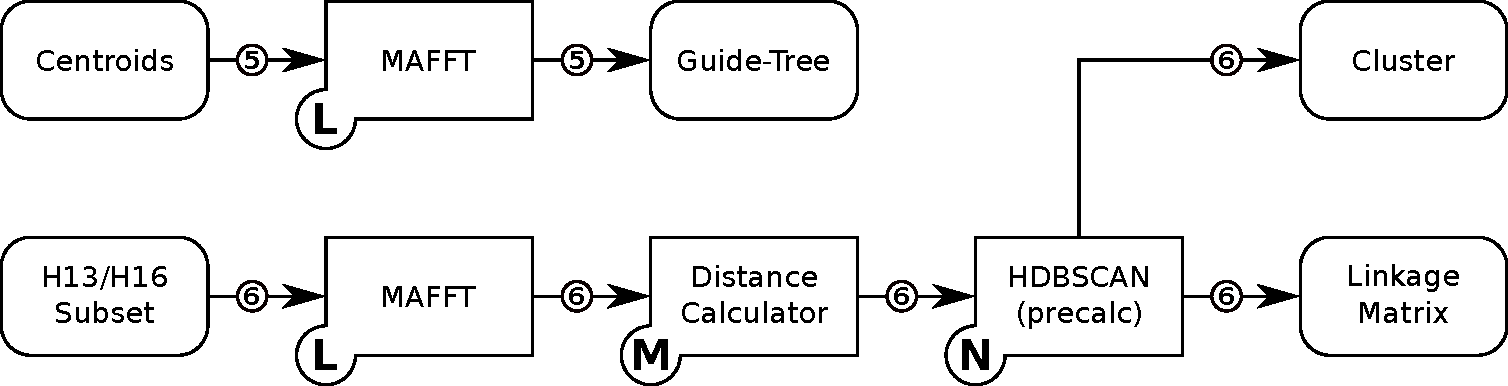
\includegraphics[width=\textwidth]{Graphics/Alignment.pdf}
    \caption[Alignment pipeline]{\textbf{Alignment pipeline.} The sequences related to the centroid vectors were aligned using \texttt{MAFFT} resulting in the output as guide-tree visualized by \texttt{ETE3} (\textsf{\textbf{L}} and pathway \textsf{\textbf{5}}). A small FASTA subset of H13/H16 was also aligned by \texttt{MAFFT} prior to evolutionary distance calculation with \texttt{BioPython} and clustering with \texttt{HDBSCAN} (\textsf{\textbf{L}}, \textsf{\textbf{M}}, \textsf{\textbf{N}} and pathway \textsf{\textbf{6}}).}
    \label{fig:Alignment_Pipeline}
\end{figure}

The precalculated trees were created using cosine distance calculation on the L1-norm normalized 7-mer frequency vectors of the segment 4 H13 and H16 sequences of the FASTA (\autoref{fig:Precalc_Pipeline} \textsf{\textbf{F}}). The calculated distances were used for \gls{UPGMA} tree building with \texttt{BioPython} (\autoref{fig:Alignment_Pipeline} \textsf{\textbf{O}} and \textsf{\textbf{P}}). The vectors were also clustered by \texttt{HDBSCAN} using the calculated distances with \texttt{metric='precalculated'}. Other settings were used as described in \autoref{sec:HDBSCAN} without hybrid clustering.

\vspace{1em}

\texttt{MAFFT} was used for \glspl{MSA} and guide tree creation with \texttt{treeout=True} on the centroid sequences and on the FASTA subset containing H13 and H16 sequences of segment 4 (\autoref{fig:Alignment_Pipeline} \textsf{\textbf{L}}) \autocite{katoh_mafft_2013}. The \gls{MSA} of the FASTA subset was converted to evolutionary distances with \texttt{BioPython} and clustered by \texttt{HDBSCAN} (\autoref{fig:Alignment_Pipeline} \textsf{\textbf{M}} and \textsf{\textbf{N}}). Pairwise alignments in \autoref{sec:Serotype_Classification} were performed using \texttt{BioPython}.